\documentclass[12pt]{report}
\usepackage[utf8]{inputenc}
\usepackage[russian]{babel}
%\usepackage[14pt]{extsizes}
\usepackage{listings}

% Для листинга кода:
\lstset{ %
language=go,                 % выбор языка для подсветки 
basicstyle=\small\sffamily, % размер и начертание шрифта для подсветки кода
numbers=left,               % где поставить нумерацию строк (слева\справа)
numberstyle=\tiny,           % размер шрифта для номеров строк
stepnumber=1,                   % размер шага между двумя номерами строк
numbersep=5pt,                % как далеко отстоят номера строк от подсвечиваемого кода
showspaces=false,            % показывать или нет пробелы специальными отступами
showstringspaces=false,      % показывать или нет пробелы в строках
showtabs=false,             % показывать или нет табуляцию в строках            
tabsize=2,                 % размер табуляции по умолчанию равен 2 пробелам
captionpos=t,              % позиция заголовка вверху [t] или внизу [b] 
breaklines=true,           % автоматически переносить строки (да\нет)
breakatwhitespace=false, % переносить строки только если есть пробел
escapeinside={\#*}{*)}   % если нужно добавить комментарии в коде
}

% Для измененных титулов глав:
\usepackage{titlesec, blindtext, color} % подключаем нужные пакеты
\definecolor{gray75}{gray}{0.75} % определяем цвет
\newcommand{\hsp}{\hspace{20pt}} % длина линии в 20pt
% titleformat определяет стиль
\titleformat{\chapter}[hang]{\Huge\bfseries}{\thechapter\hsp\textcolor{gray75}{|}\hsp}{0pt}{\Huge\bfseries}


% plot
\usepackage{pgfplots}
\usepackage{filecontents}
\usepackage{amsmath}
\usepackage{tikz,pgfplots}
\usetikzlibrary{datavisualization}
\usetikzlibrary{datavisualization.formats.functions}

\begin{filecontents}{one.dat}
100  0.0049889
200 0.047874
300 0.16655
400 0.373
500 1.2694
600 1.4870
700 2.7989
800 4.825
900 13.69
1000 20.373
\end{filecontents}
\begin{filecontents}{two.dat}
100  0.002
200 0.029
300 0.081
400 0.264
500 0.669
600 0.7689
700 1.4482
800 2.2068
900 7.97
1000 11.3583
\end{filecontents}
\begin{filecontents}{four.dat}
100  0.0019
200 0.01894
300 0.067
400 0.176
500 0.457
600 0.579
700 1.01
800 1.62
900 5.83
1000 8.334
\end{filecontents}

\begin{filecontents}{six.dat}
100  0.003
200 0.02
300 0.07
400 0.163
500 0.432
600 0.567
700 1.07
800 1.65
900 6.06
1000 8.071
\end{filecontents}
\begin{filecontents}{eight.dat}
100  0.00199
200 0.025
300 0.07
400 0.157
500 0.467
600 0.568
700 1.04
800 1.73
900	5.76
1000 8.08
\end{filecontents}

\usepackage{graphicx}
\graphicspath{{src/}}
\DeclareGraphicsExtensions{.pdf,.png,.jpg}

\begin{document}
%\def\chaptername{} % убирает "Глава"
\begin{titlepage}
	\centering
	{\scshape\LARGE МГТУ им. Баумана \par}
	\vspace{3cm}
	{\scshape\Large Лабораторная работа №2\par}
	\vspace{0.5cm}	
	{\scshape\Large По курсу: "Анализ алгоритмов"\par}
	\vspace{1.5cm}
	{\huge\bfseries Параллельное умножение матриц\par}
	\vspace{2cm}
	\Large Работу выполнил: Мокеев Даниил, ИУ7-54\par
	\vspace{0.5cm}
	\Large Преподаватели:  Волкова Л.Л., Строганов Ю.В.\par

	\vfill
	\large \textit {Москва, 2019} \par
\end{titlepage}

\tableofcontents

\newpage
\chapter*{Введение}
\addcontentsline{toc}{chapter}{Введение}

Цель работы: изучение возможности параллельных вычислений и использование такого подхода на практике. Реализация парралельного алгоритма Винограда умножения матриц. В данной лабораторной работе рассматривается алгоритм Винограда и параллельный алгоритм Винограда. Необходимо сравнить зависимость времени работы алгоритма от числа параллельных потоков и размера матриц, провести сравнение стандартного и параллельного алгоритмов.

В ходе лабораторной работы предстоит:
\begin{itemize}
	\item изучить алгоритмы умножения матриц: стандартный и алгоритм Винограда; 
	\item оптимизировать алгоритм Винограда; 
	\item дать теоретическую оценку базового алгоритма умножения матриц, алгоритма Винограда и улучшенного алгоритма Винограда;
	\item реализовать три алгоритма умножения матриц на одном из языков программирования;  
	\item сравнить алгоритмы умножения матриц.
\end{itemize}

\chapter{Аналитическая часть}
Матрицей A размера $[m*n]$ называется прямоугольная таблица
чисел, функций или алгебраических выражений, содержащая m строк и n столбцов. Числа m и n определяют размер матрицы.\cite{Beloysov} Если число столбцов в первой матрице совпадает с числом строк во второй, то эти две матрицы можно перемножить. У произведения будет столько же строк, сколько в первой матрице, и столько же столбцов, сколько во второй.

Пусть даны две прямоугольные матрицы А и В размеров $[m * n]$ и $[n * k]$ соответственно.  
В результате произведение матриц A и B получим матрицу C размера $[m *  k]$.


$c_{i,j} = \sum\limits_{r=1}^n a_{i,r}\cdot b_{r,j}$ называется произведением матриц A и B \cite{Beloysov}.


\section{Алгоритм Винограда}
Подход Алгоритма Винограда является иллюстрацией общей методологии, начатой в 1979-х годах на основе
билинейных и трилинейных форм, благодаря которым большинство усовершенствований для умножения матриц были получены \cite{Gall2012}.

Рассмотрим два вектора $V = (v1, v2, v3, v4)$ и $W = (w1, w2, w3, w4)$.  

Их скалярное произведение равно (\ref{formula}) 

\begin{equation} \label{formula}
V \cdot W=v_1 \cdot w_1 + v_2 \cdot w_2 + v_3 \cdot w_3 + v_4 \cdot w_4
\end{equation}

Равенство (\ref{formula}) можно переписать в виде(\ref{formula2}) 
\begin{equation} \label{formula2}
V \cdot W=(v_1 + w_2) \cdot (v_2 + w_1) + (v_3 + w_4) \cdot (v_4 + w_3) - v_1 \cdot v_2 - v_3 \cdot v_4 - w_1 \cdot w_2 - w_3 \cdot w_4
\end{equation}

Менее очевидно, что выражение в правой части последнего равенства допускает предварительную обработку: его части можно вычислить заранее и запомнить для каждой строки первой матрицы и для каждого столбца второй. 
Это означает, что над предварительно обработанными элементами нам придется выполнять лишь первые два умножения и последующие пять сложений, а также дополнительно два сложения. 

\subsection{Параллельный алгоритм Винограда}
Трудоемкость алгоритма Винограда имеет сложность $O(nmk)$ для умножения матриц $n1 \times m1$ на $n2 \times m2$. Чтобы улучшить алгоритм, следует распараллелить ту часть алгоритма, которая содержит 3 вложенных цикла.\\

Вычисление результата для каждой строки не зависит от результата выполнения умножения для других строк. Поэтому можно распараллелить часть кода, где происходят эти действия. Каждый поток будет выполнять вычисления определенных строк результирующей матрицы.

\section{Параллельное программирование}

При использовании многопроцессорных вычислительных систем с общей памятью обычно предполагается, что имеющиеся в составе системы процессоры обладают равной производительностью, являются равноправными при доступе к общей памяти, и время доступа к памяти является одинаковым (при одновременном доступе нескольких процессоров к одному и тому же элементу памяти очередность и синхронизация доступа обеспечивается на аппаратном уровне). Многопроцессорные системы подобного типа обычно именуются симметричными мультипроцессорами (symmetric multiprocessors, SMP).

Перечисленному выше набору предположений удовлетворяют также активно развиваемые в последнее время многоядерные процессоры, в которых каждое ядро представляет практически независимо функциони рующее вычислительное устройство.

Обычный подход при организации вычислений для многопроцессорных вычислительных систем с общей памятью – создание новых параллельных методов на основе обычных последовательных программ, в которых или автоматически компилятором, или непосредственно программистом выделяются участки независимых друг от друга вычислений. Возможности автоматического анализа программ для порождения параллельных вычислений достаточно ограничены, и второй подход является преобладающим. При этом для разработки параллельных программ могут применяться как новые алгоритмические языки, ориентированные на параллельное программирование, так и уже имеющиеся языки, расширенные некоторым набором операторов для параллельных вычислений.

Широко используемый подход состоит и в применении тех или иных библиотек, обеспечивающих определенный программный интерфейс (application programming interface, API) для разработки параллельных программ. В рамках такого подхода наиболее известны Windows Thread API. Однако первый способ применим только для ОС семейства Microsoft Windows, а второй вариант API является достаточно трудоемким для использования и имеет низкоуровневый характер \cite{Barkalov}.

\subsection{Организация взаимодействия параллельных потоков}
Потоки исполняются в общем адресном пространстве параллельной программы. Как результат, взаимодействие параллельных потоков можно организовать через использование общих данных, являющихся доступными для всех потоков. Наиболее простая ситуация состоит в использовании общих данных только для чтения. В случае же, когда общие данные могут изменяться несколькими потоками, необходимы специальные усилия для организации правильного взаимодействия.


\section{Вывод}
Был рассмотрен алгоритм Винограда и возможность его оптимизации с помощью распараллеливания потоков. Была рассмотрена технология параллельного программирования и
организация взаимодействия параллельных потоков.

\chapter{Конструкторская часть}
\textbf{Требования к вводу:}
На вход подаются две матрицы
\newline
\textbf{Требования к программе:}
\begin{itemize}
	\item корректное умножение двух матриц;
	\item при матрицах неправильных размеров программа не должна аварийно завершаться.
\end{itemize}

\section{Схемы алгоритмов}
В данной части будут рассмотрена схема алгоритма Винограда.

\begin{figure}[!htbp]
	\centering
	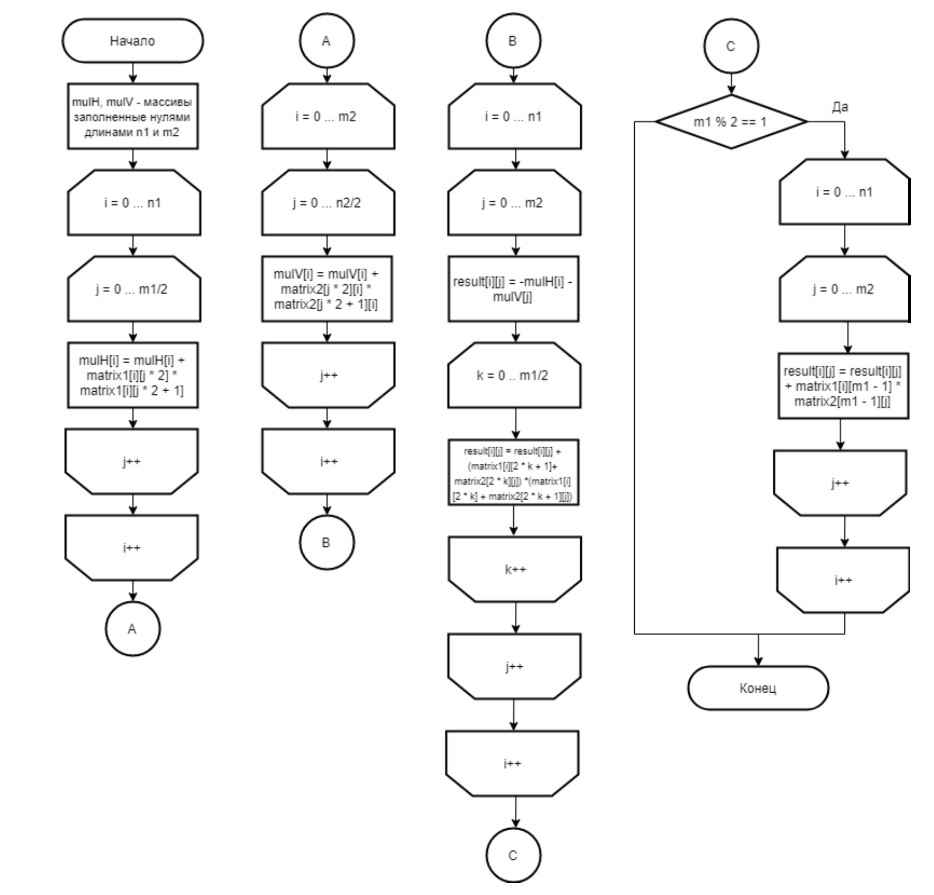
\includegraphics[width=1.3\linewidth]{winograd.png}
	\caption{Схема алгоритма Винограда}
	\label{fig:winogr}
\end{figure}

\section{Распараллеливание программы}
Распрараллеливание программы должно ускорять время работы. Это достигается за счет реализации в узких участках (напимер в циклах с большим количеством независимых вычилений).

В предложенном алгоритме данным участком будет являться тройной цикл поиска результата.
Данный блок программы как раз предлагается распараллелить.
На (Рис. 2.1) это участок между B и С. 

\section{Вывод}
В данном разделе была рассмотрена схема алгоритма Винограда и способ ее распараллеливания.

\chapter{Технологическая часть}
\section{Выбор ЯП}
Я выбрал в качестве языка программирования Golang, потому как он достаточно удобен, быстр и успешно использует концепции мультипоточного программирования.

Время работы алгоритмов было замерено с помощью функции Now() из библиотеки time.

\section{Описание структуры ПО}
В данном разделе будет представленна функциональная схема программы (Рис. 3.1.)
\begin{figure}[h]
	\centering
	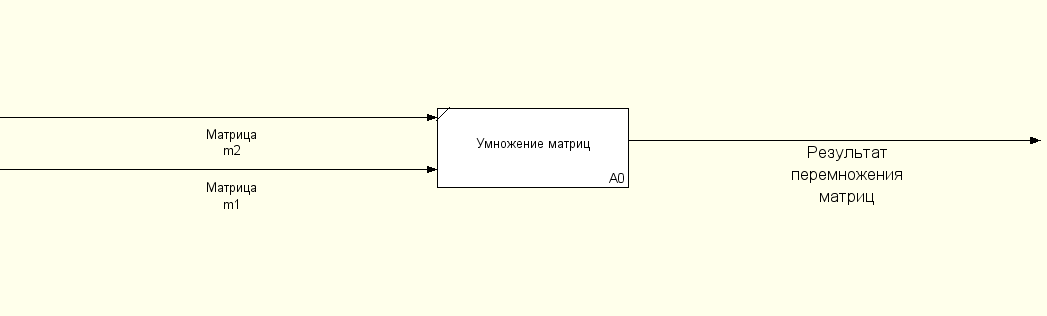
\includegraphics[width=1.25\linewidth]{lab02ram}
	\caption{Функциональная схема умножения матриц (IDEF0 диаграмма 1 уровня)}
	\label{fig:mpr}
\end{figure}

\section{Сведения о модулях программы}
Программа состоит из:
\begin{itemize}
	\item lab04.go- главный файл программы, в котором располагается точка входа в программу.
	\item matr.go - файл содержащий функции предобработки матриц и измерение времени.
\end{itemize}

\section{Листинг кода алгоритмов}
В данном разделе будет представлен листинги кода алгоритма Винограда (3.1), распараллеленого алгоритма Винограда (3.2)
\begin{lstlisting}[label=CodeStand,caption = Алгоритм Винограда]
func winograd(mtr1, mtr2 *mtr) *mtr{
	if mtr2.rows != mtr1.cols{
		panic("Wrong size of matrix")
	}
	row1 := mtr1.rows; col1 := mtr1.cols
	row2:= mtr2.rows; col2 := mtr2.cols

	row_factor := make([]int, row1, row1)
	col_factor := make([]int, col2, col2)

	for i:=0; i<row1;i++{
		for j:=0;j<col1 / 2;j++{
			row_factor[i] += mtr1.buff[i][2*j] * mtr1.buff[i][2*j+1]
	}}
	
	for i:=0; i<col2;i++{
		for j:=0;j<row2 / 2;j++{
			col_factor[i] += mtr2.buff[2*j][i]*mtr2.buff[2*j+1][i]
	}}

		answer := new_mtr(row1, col2)

	for i:=0;i<row1;i++{
		for j:=0;j<col2;j++{
			answer.buff[i][j]+= - row_factor[i] - col_factor[j]
			for k:=0;k<col1 / 2;k++{
				answer.buff[i][j] += ((mtr1.buff[i][2 * k] + mtr2.buff[2 * k + 1][j]) * (mtr1.buff[i][2 * k + 1] + mtr2.buff[2 * k][j]))
	}}}

	if (row2 % 2) != 0{
		for i:=0;i<row1;i++{
			for j:=0;j<col2;j++{
				answer.buff[i][j] += mtr1.buff[i][col1 - 1] * mtr2.buff[col1 - 1][j]
	}}}
	return answer
}
\end{lstlisting}

\begin{lstlisting}[label=winograd_mult,caption=Распараллеленый Алгоритм Винограда]
func winograd_parallel(mtr1, mtr2 *mtr, threads int) *mtr{
	if mtr2.rows != mtr1.cols{
		panic("Wrong size of matrix")
	}
	row1 := mtr1.rows; col1 := mtr1.cols
	row2:= mtr2.rows; col2 := mtr2.cols

	row_factor := make([]int, row1, row1)
	col_factor := make([]int, col2, col2)

	for i:=0; i<row1;i++{
		for j:=0;j<col1 / 2;j++{
			row_factor[i] += mtr1.buff[i][2*j] * mtr1.buff[i][2*j+1]
	}}
	for i:=0; i<col2;i++{
		for j:=0;j<row2 / 2;j++{
			col_factor[i] += mtr2.buff[2*j][i]*mtr2.buff[2*j+1][i]
	}}
	answer := new_mtr(row1, col2)
	in := make(chan int); quit := make(chan bool)
	mult := func(){
		for{
			select {
				case i := <- in:
					for j:=0;j<col2;j++{
					answer.buff[i][j]+= - row_factor[i] - col_factor[j]
					for k:=0;k<col1 / 2;k++{
					answer.buff[i][j] += ((mtr1.buff[i][2 * k] + mtr2.buff[2 * k + 1][j]) * (mtr1.buff[i][2 * k + 1] + mtr2.buff[2 * k][j]))
					}}
			case <- quit:
				return
			}
		}
	}
	for i:=0;i<threads;i++{
		go mult()
	}
	for i:=0;i<mtr1.rows;i++{
		in <- i
	}
	for i:= 0 ; i<threads; i++{
		quit<-true
	}
	return answer
}
\end{lstlisting}


\section{Вывод}
В данном разделе была рассмотрена структура ПО и листинги кода программы.

\chapter{Исследовательская часть}
Был проведен замер времени работы алгоритмов с использованием разного колличества потоков.
Исследования были проведены на процессоре Intel Core i5-6200U
\section{Примеры работы}
В данном разделе приведен пример работы программы (Рис. 4.1)
\begin{figure}[h]
	\centering{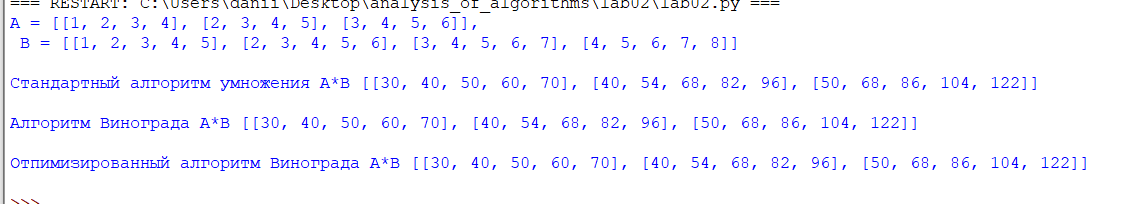
\includegraphics[scale=1.1]{example.png}} 
	\caption{Пример работы программы}
	\label{ris:example}
\end{figure}

\section{Постановка эксперемента}
Проведем сравнение для каждого из алгоритмов. Для замера времени будем использовать функцию time.Now()

Сравним результаты для обычного Винограда и Винограда с распараллеленным главным циклом:
\newpage

\begin{figure}
\begin{tikzpicture}[thick, scale=1.4]
\begin{axis}[
    	axis lines = left,
    	xlabel = $size$,
    	ylabel = {$time(sec)$},
	legend pos=north west,
	ymajorgrids=true
]
\addplot[color=red] table[x index=0, y index=1] {winograd.dat}; 
\addplot[color=green] table[x index=0, y index=1] {one.dat};
\addplot[color=blue, mark=square] table[x index=0, y index=1] {two.dat};
\addplot[color=brown] table[x index=0, y index=1] {four.dat}; 
\addplot[color=orange] table[x index=0, y index=1] {six.dat};
\addplot[color=black, mark=square] table[x index=0, y index=1] {eight.dat};

\addlegendentry{Обычный Виноград}
\addlegendentry{1 thread}
\addlegendentry{2 threads}
\addlegendentry{4 threads}
\addlegendentry{6 threads}
\addlegendentry{8 threads}
\end{axis}
\end{tikzpicture}
\caption{Сравнение использования разного количества потоков} \label{plot:even}
\end{figure}
\par

\newpage
\subsection{Вывод эксперементальной части}
Экперемент показывает, что использование одного потока эквивалентно обычной версии алгоритма. Использование двух потоков значительно ускоряет работу алгоритма. Данный эффект наблюдается и при увеличении числа потоков, однако при использовании более четырех потоков дальнейшего ускорения не происходит.
\chapter*{Заключение}
\addcontentsline{toc}{chapter}{Заключение}
В ходе лабораторной работы были изучены возможности параллельных вычислений, реализован алгоритм Винограда умножения матриц
с помощью параллельных вычислений.

Было произведено сравнение работы обычного алгоритма Винограда и параллельной реализации при увеличении количества потоков. Выяснилось, что увеличение потоков до 4х сокращает время работы на 70\% по сравнению с
однопоточной реализацией. Однако дальнейшее увеличение количества потоков не дает значительного выигрыша во времени (разница менее 1\%). 

\addcontentsline{toc}{chapter}{Список литературы}
\begin{thebibliography}{3}
	\bibitem{Beloysov}
	И. В. Белоусов(2006), Матрицы и определители, учебное пособие по линейной алгебре, с. 1 - 16
	\bibitem{Gall2012}
	Le Gall, F. (2012), "Faster algorithms for rectangular matrix multiplication", Proceedings of the 53rd Annual IEEE Symposium on Foundations of Computer Science (FOCS 2012), pp. 514–523
	%https://arxiv.org/pdf/1204.1111.pdf
	\bibitem{Barkalov}
	Константин Баркалов, Владимир Воеводин, Виктор Гергель. Intel Parallel Programming [Электронный ресурс], - режим доступа https://www.intuit.ru/studies/courses/4447/983/lecture/14925
	\bibitem{Microsoft}
	Руководство по языку C\#[Электронный ресурс], - режим доступа: https://docs.microsoft.com/ru-ru/dotnet/csharp/
\end{thebibliography}

\end{document}

